
\subsection{Dealing with uncertain labels}
\begin{frame}
\begin{quote}
...all clinically diagnosed AD patients will not have AD pathology, and up to 30\% of cognitively normal subjects will have a pathologic diagnosis of AD at autopsy.
\end{quote}

\begin{center}\begin{tiny}
Vemuri et al. ``Antemortem MRI based STructural Abnormality iNDex (STAND)-scores correlate with postmortem Braak neurofibrillary tangle stage''. NeuroImage 42(2):559--567 (2008).

\end{tiny}\end{center}
\end{frame}


\subsection{Visualising differences}

\begin{frame}
\frametitle{Visualising differences}
Neuroimagers like their blobs and summary tables.

How do we best understand whole-brain multivariate differences?

Here's my attempt.....
\end{frame}



\begin{frame}
\frametitle{Exaggerated male brain}
\begin{center}
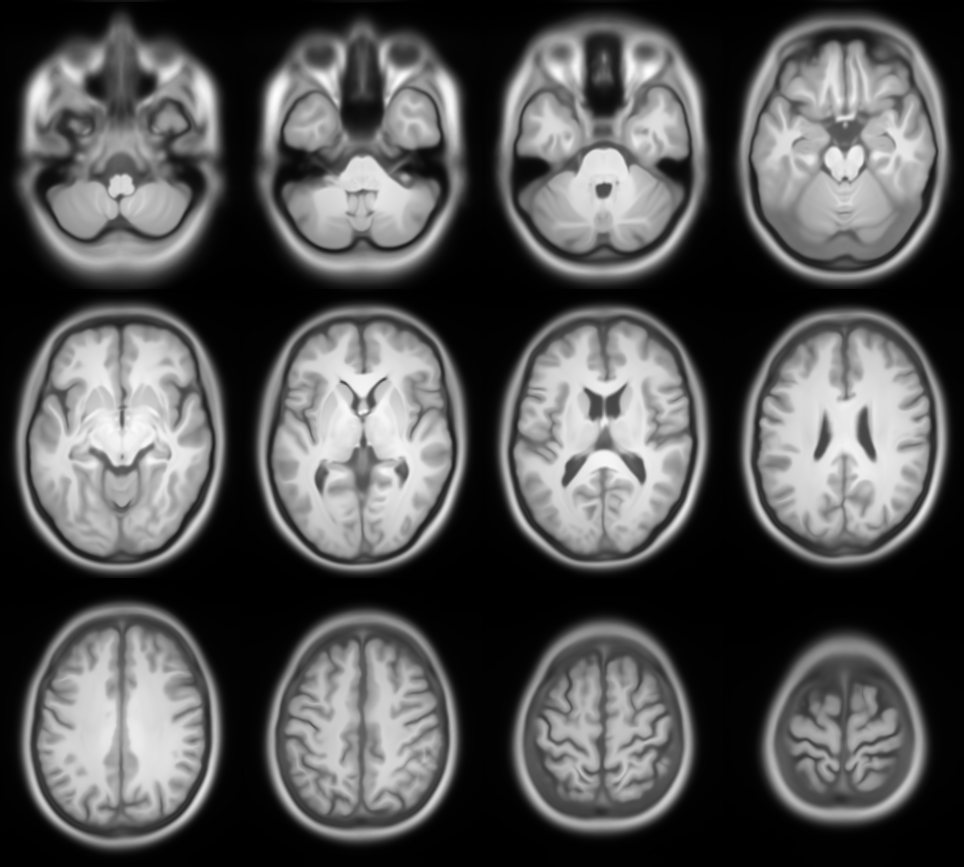
\includegraphics[width=.7\textwidth]{hyper_male}
\end{center}
\end{frame}



\begin{frame}
\frametitle{Average brain}
\begin{center}
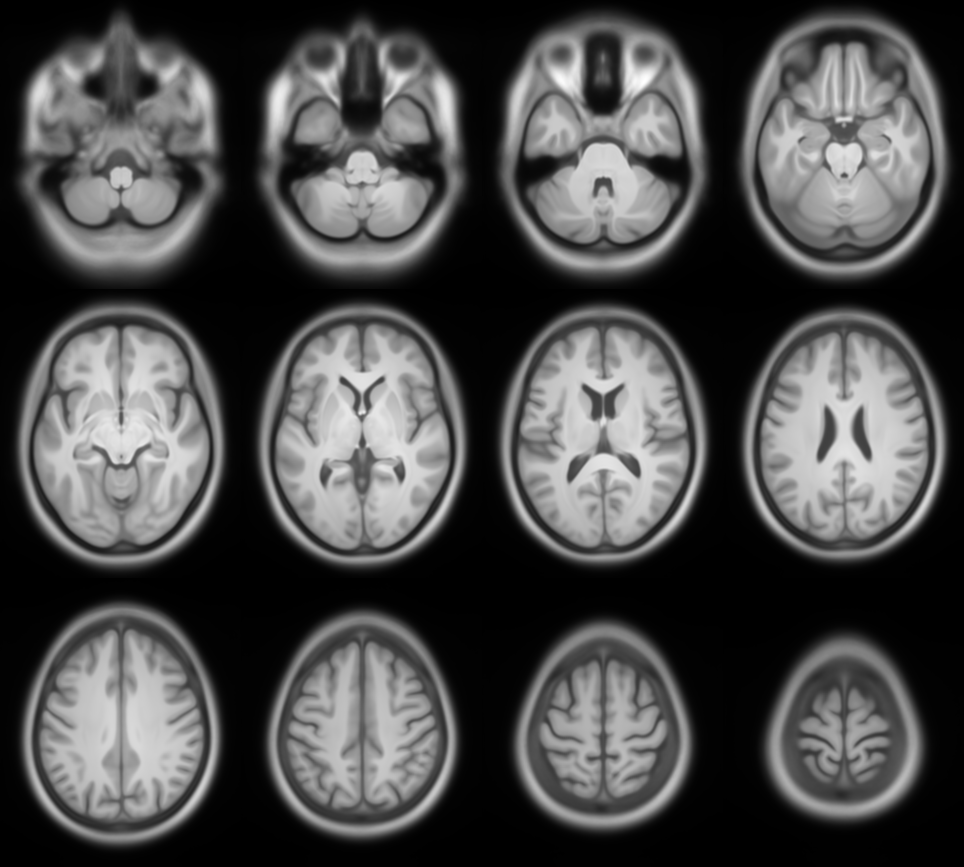
\includegraphics[width=.7\textwidth]{avgT1}
\end{center}
\end{frame}



\begin{frame}
\frametitle{Exaggerated female brain}
\begin{center}
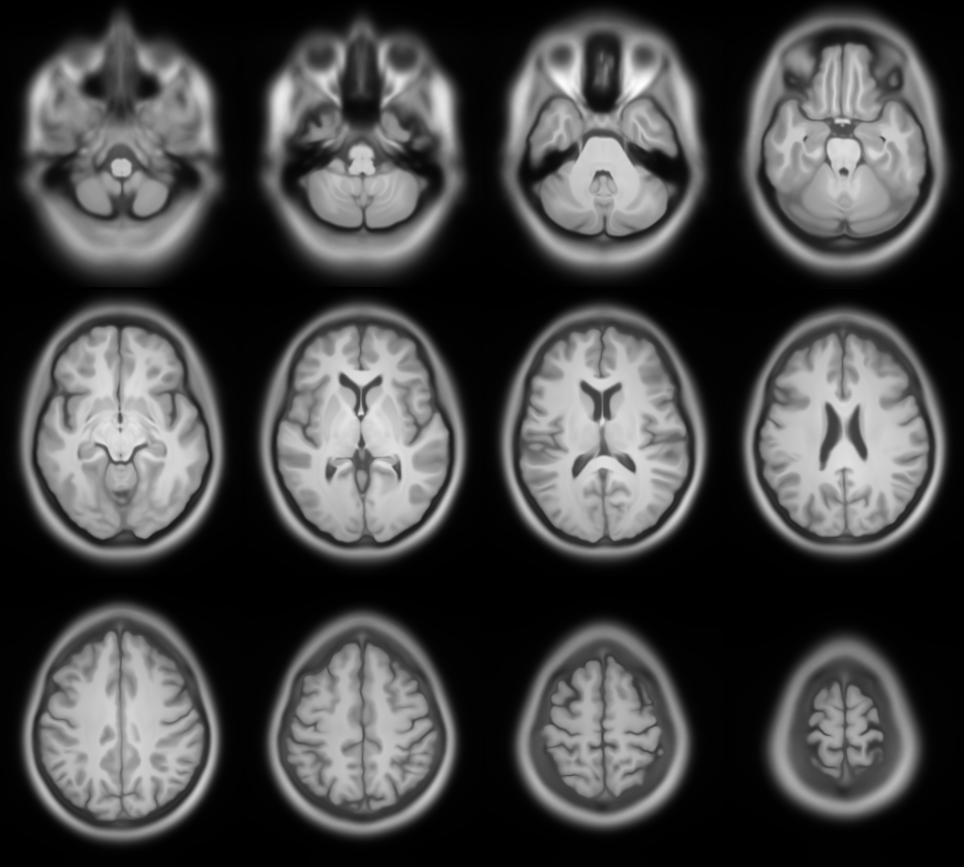
\includegraphics[width=.7\textwidth]{hyper_female}
\end{center}
\end{frame}

